\documentclass{article}
\usepackage[italian]{babel}
\usepackage{graphicx}
\usepackage{enumerate}
\usepackage{float}
\usepackage[table]{xcolor}
\usepackage{subcaption}
\usepackage{verbatim} 
\usepackage{amsmath}
\usepackage{xcolor,colortbl}
\usepackage{adjustbox}
\usepackage{framed}
\usepackage[hidelinks]{hyperref}
\usepackage[a4paper,top=2cm,bottom=2cm,left=3cm,right=3cm,marginparwidth=1.75cm]{geometry}

\definecolor{Gray}{gray}{0.5}
\definecolor{LightGray}{gray}{0.8}

\title{PROGETTO BASI DI DATI}
\author{Giovanni Manfredi}
\date{2022-2023}
\begin{document}

\maketitle
\tableofcontents

\section{Introduzione}
\subsection{Analisi iniziale}
La seguente documentazione specifica nel dettaglio il dominio applicativo d'interesse e serve ad analizzare nel modo più preciso possibile tutti gli aspetti che lo riguardano.

\subsection{Traccia}
La \textbf{Federazione Internazionale dell'Automobile} (FIA) intende tener traccia dei campionati mondiali di Formula 1. Ogni anno si apre con l'inaugurazione del mondiale di cui si vuole tener traccia. Ogni mondiale è caratterizzato dell'edizione, che identifica ogni mondiale, dal regolamento, da una descrizione formale e dal numero di auto partecipanti. In ciascun mondiale partecipano delle scuderie e, per ognuna di esse, si vuole tener traccia: del nome (univoco per ogni scuderia), dell'anno di fondazione e dei team che ci lavorano. Ogni team è caratterizzato dal settore ricoperto il quale, assieme alla scuderia di appartenenza, è in grado d'identificare univocamente ogni team; questo è possibile in quanto non vi possono essere più team all'interno di una scuderia che ricoprono lo stesso settore. In ogni mondiale partecipano al più 10 scuderie e, per ogni scuderia, i team sviluppano 2 vetture. Le vetture sono obbligatoriamente diverse ogni anno e, pertanto, è possibile identificarle in base all'edizione del mondiale e al numero in gara (diverso per ogni vettura). Inoltre, ciascuna vettura, si compone anche di nome e numero di cavalli e, per ogni singola vettura in competizione, potrebbero esse necessari dei commenti. 

Dei dipendenti che lavorano per i team si vuole tener traccia: della matricola, del nome, del cognome e della data di nascita. Fra le tipologie di dipendenti siamo interessati a: Team principal e Piloti. Dei team principal si vuole memorizzare il numero di anni di esperienza mentre, per i piloti, per questioni regolamentari, bisogna conservare anche il BMI (Body Mass Index) composto da peso e l'altezza.
I piloti candidati per le gare otterranno al termine di ogni gara: una posizione finale e il relativo punteggio. I piloti gareggeranno su dei tracciati identificati dal nome e caratterizzati dalla nazione di appartenenza; un pilota può gareggia più volte sullo stesso circuito.
\section{Progettazione concettuale}
Il seguente schema ER è stato ottenuto seguendo una strategia \textbf{top-down}.

\subsection{Schema ER}
\begin{figure}[H]
    \centering
    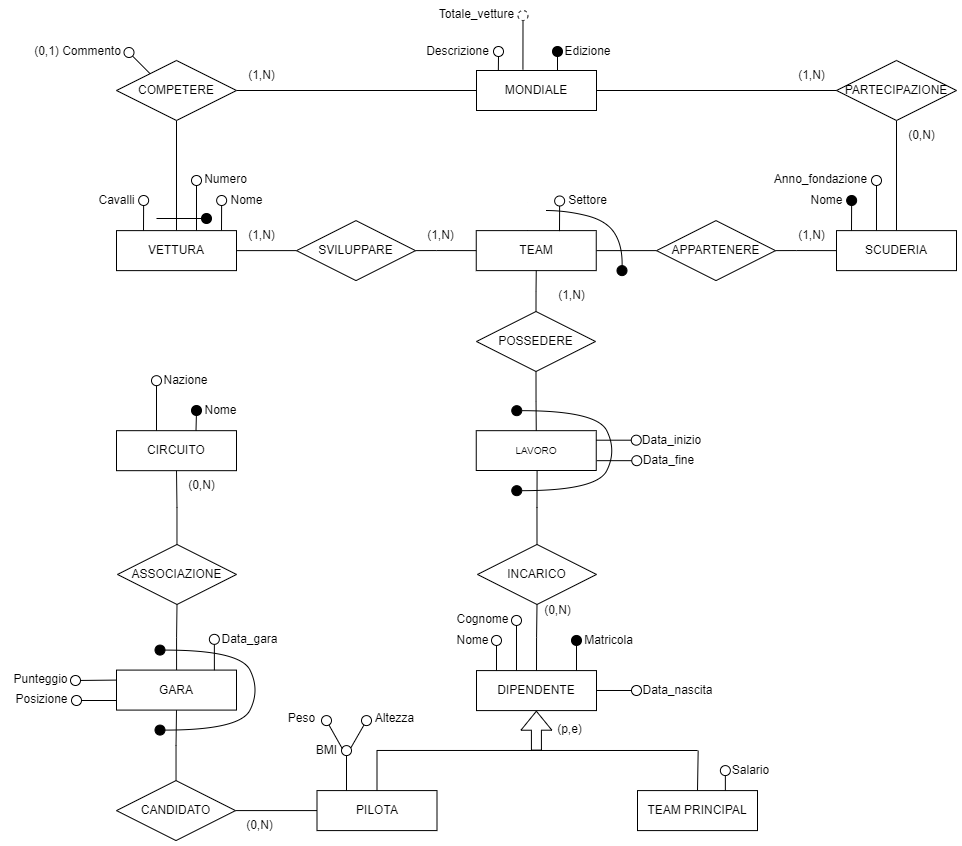
\includegraphics[scale = 0.73]{Images/ER.png}
\end{figure}

\newpage
\subsection{Business rules}
Passiamo adesso alla documentazione di supporto creando un'interpretazione personale dello schema e descrivendo le proprietà dei dati rappresentati.

\subsubsection{Descrizione dei concetti}

\begin{figure}[H]
    \centering
    \includegraphics[scale = 0.74]{Images/Table/Dizionario dei dati - entità dello schema.png}
\end{figure}


\begin{figure}[H]
    \centering
    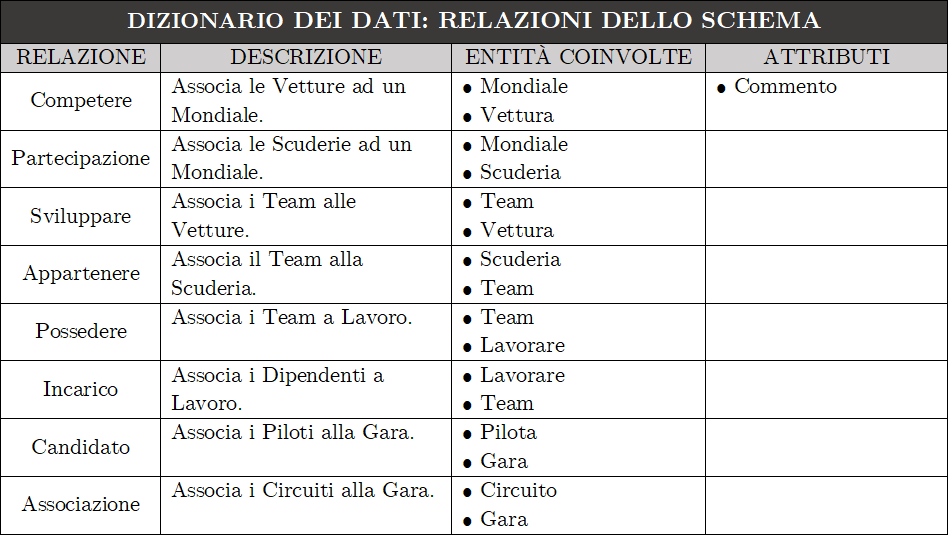
\includegraphics[scale = 0.74]{Images/Table/Dizionario dei dati - relazioni dello schema.png}
\end{figure}


\subsection{Vincoli d'integrità}
\begin{itemize}
    \item[$\diamondsuit$]  In un mondiale devono partecipare minimo 1 scuderia e massimo 10;
    \item[$\diamondsuit$] Una scuderia non deve partecipare allo stesso mondiale più di 1 volta;
    \item[$\diamondsuit$] Un team deve sviluppare minimo 1 vettura e 2 due;
    \item[$\diamondsuit$] Una vettura non deve partecipare a più di un mondiale;
    \item[$\diamondsuit$] Un pilota deve essere candidato ad almeno una gara;
    \item[$\diamondsuit$] In un circuito non devono esserci più gare nello stesso momento.
\end{itemize}

\subsection{Derivazioni}
\begin{itemize}
    \item[$\diamondsuit$] Il numero totale delle vetture che hanno partecipato ai mondiali si ottiene contando il numero di relazioni tra Mondiale e Vettura.
\end{itemize}

\subsection{Carico applicativo}

\subsubsection{Tavola dei volumi}
\begin{figure}[H]
    \centering
    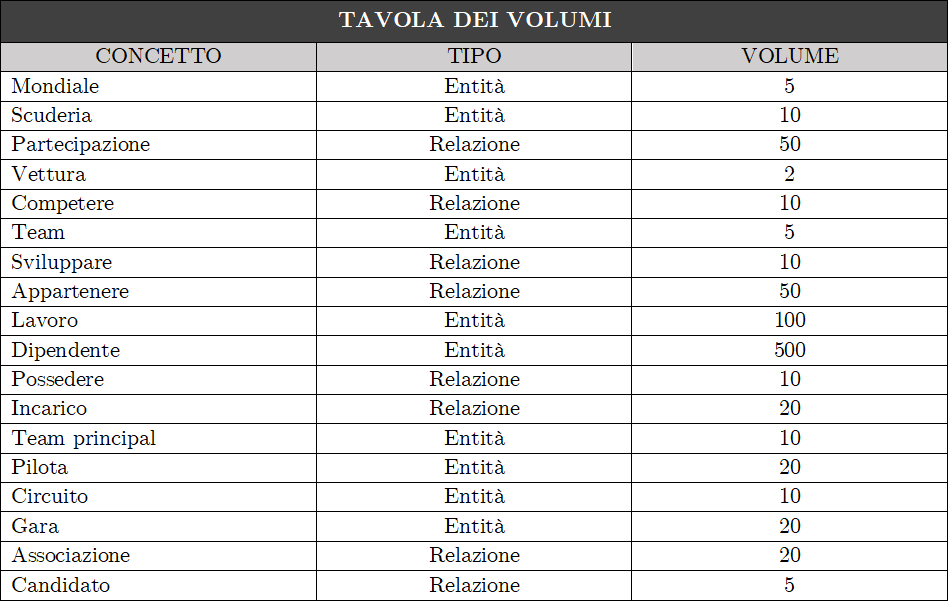
\includegraphics[scale = 0.74]{Images/Table/Tavola volumi.png}
\end{figure}

\subsubsection{Tavola delle operazioni}
\begin{figure}[H]
    \centering
    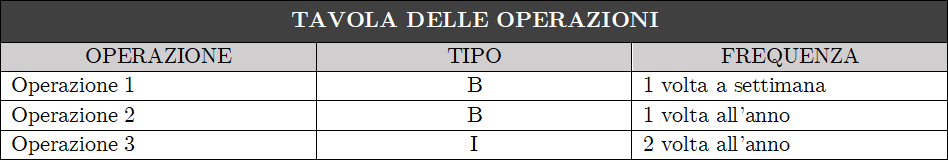
\includegraphics[scale = 0.74]{Images/Table/Tavola operazioni.png}
\end{figure}

\begin{itemize}
    \item \textbf{Operazione 1:} Generazione della classifica;
    \item \textbf{Operazione 2:} Visualizzazione del numero totale di macchine partecipanti al mondiale;
    \item \textbf{Operazione 3:} Inserimento di un nuovo circuito.
\end{itemize}

\subsubsection{Tavole degli accessi}

\begin{figure}[H]
    \centering
    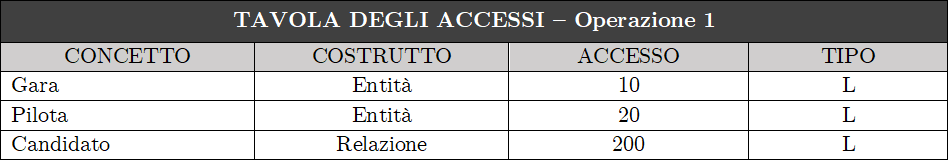
\includegraphics[scale = 0.74]{Images/Table/Tavola accessi - op1.png}
\end{figure}

\begin{equation*}
    230L \cdot 4 = 920L \cdot 12 = 11040L
\end{equation*}

In totale abbiamo 144 accessi annui il che potrebbe farci pensare di \emph{conservare}, creando un entità, la classifica all'interno del DataBase.

\begin{figure}[H]
    \centering
    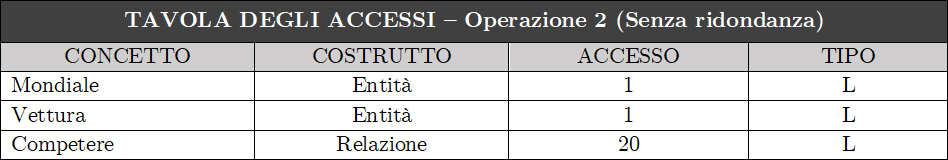
\includegraphics[scale = 0.74]{Images/Table/Tavola accessi - op2.png}
\end{figure}

\begin{equation*}
    22L
\end{equation*}

Passiamo adesso ad analizzare la tavola degli accessi mantenendo l'attributo \emph{Totale$\_$vetture} ridondante:

\begin{figure}[H]
    \centering
    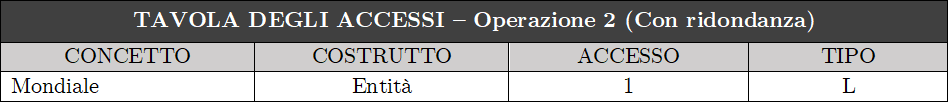
\includegraphics[scale = 0.74]{Images/Table/Tavola accessi - op2 (ridondanza).png}
\end{figure}

\begin{equation*}
    1L + 1Byte
\end{equation*}

Dall'analisi degli accessi si può notare come il mantenimento dell'attributo è conveniente e quindi si può lasciare all'interno dello schema.

\begin{figure}[H]
    \centering
    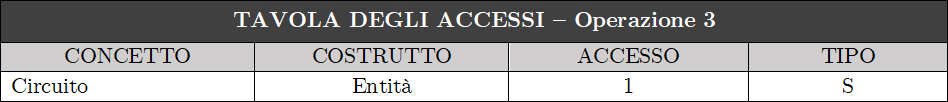
\includegraphics[scale = 0.74]{Images/Table/Tavola accessi - op3.png}
\end{figure}

\begin{equation*}
    1S = 2L
\end{equation*}
\section{Progettazione logica}
\subsection{Ristrutturazione dello schema ER}

\subsubsection{Schema ER ristrutturato}

\begin{figure}[H]
    \centering
    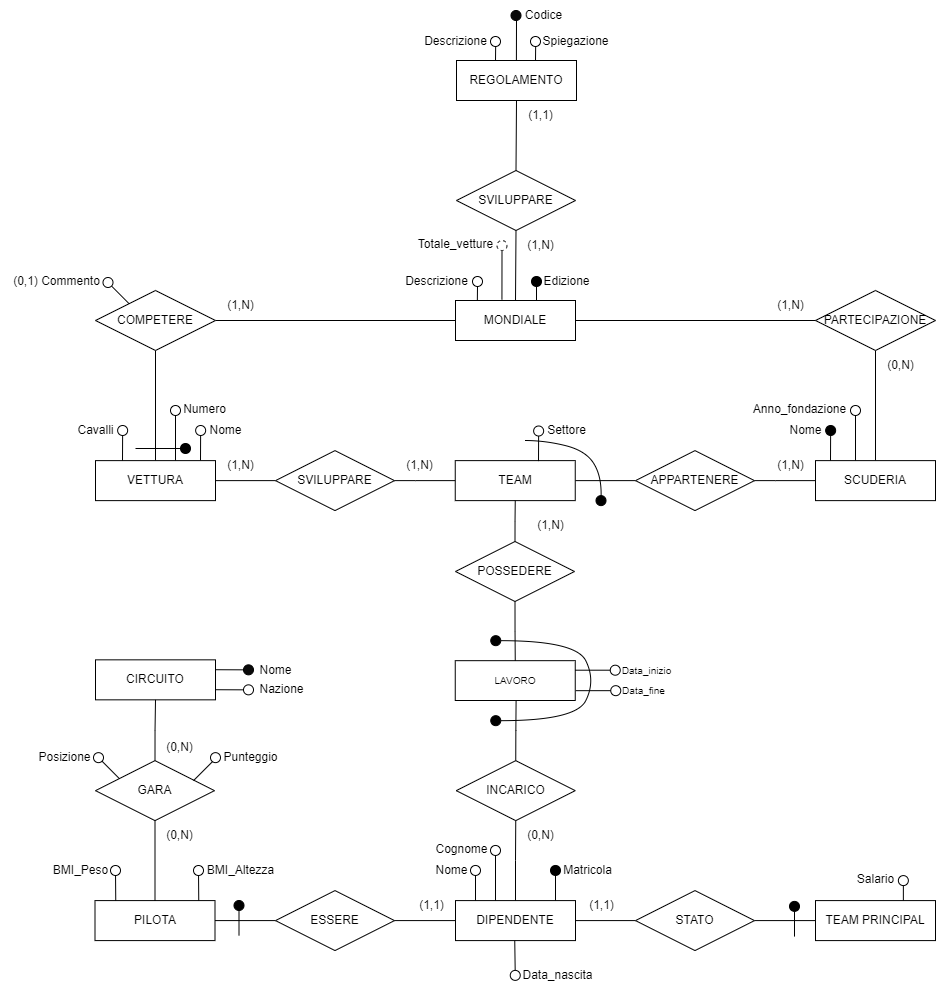
\includegraphics[scale = 0.45]{Images/ER - Ristrutturato.png}
\end{figure}

\newpage
\subsection{Traduzione verso il modello logico}

\subsubsection{Schema logico}
\begin{itemize}
    \item[$\circ$] \texttt{Mondiale (\underline{Edizione}, Descrizione)}
    \item[$\circ$] \texttt{Regolamento (\underline{Codice}, Spiegazione, Descrizione, Mondiale)}
    \item[$\circ$] \texttt{Scuderia (\underline{Nome}, Anno$\_$fondazione)}
    \item[$\circ$] \texttt{Partecipazione (\underline{Mondiale}, \underline{Scuderia})}
    \item[$\circ$] \texttt{Team (\underline{Scuderia}, \underline{Settore}, Numero$\_$dipendenti)}
    \item[$\circ$] \texttt{Vettura (\underline{Mondiale}, \underline{Numero}, Nome, Cavalli, Commento*)}
    \item[$\circ$] \texttt{Sviluppare (\underline{Vettura}, \underline{Team})}
    \item[$\circ$] \texttt{Dipendente (\underline{Matricola}, Nome, Cognome, Data$\_$nascita)}
    \item[$\circ$] \texttt{Lavoro (\underline{Team}, \underline{Dipendente}, Data$\_$inizio, Data$\_$fine)}
    \item[$\circ$] \texttt{Team principal (\underline{Dipendente}, Salario)}
    \item[$\circ$] \texttt{Pilota (\underline{Dipendente}, BMI$\_$peso, BMI$\_$altezza)}
    \item[$\circ$] \texttt{Circuito (\underline{Nome}, Nazione)}
    \item[$\circ$] \texttt{Gara (\underline{Circuito}, \underline{Pilota},\underline{Data$\_$gara}, Posizione, Punteggio)}
\end{itemize}

\vspace*{10 pt}
\noindent Con \textbf{vincoli d'integrità referenziali}:

\begin{itemize}
    \item \emph{Mondiale} in \textbf{Regolamento} con la chiave primaria di \textbf{Mondiale};
    \item \emph{Mondiale} in \textbf{Partecipazione} con la chiave primaria di \textbf{Mondiale};
    \item \emph{Scuderia} in \textbf{Partecipazione} con la chiave primaria di \textbf{Scuderia};
    \item \emph{Scuderia} in \textbf{Team} con la chiave primaria di \textbf{Scuderia};
    \item \emph{Scuderia} in \textbf{Team} con la chiave primaria di \textbf{Scuderia};
    \item \emph{Mondiale} in \textbf{Vettura} con la chiave primaria di \textbf{Mondiale};
    \item \emph{Vettura} in \textbf{Sviluppare} con la chiave primaria di \textbf{Vettura};
    \item \emph{Team} in \textbf{Sviluppare} con la chiave primaria di \textbf{Team};
    \item \emph{Team} in \textbf{Lavoro} con la chiave primaria di \textbf{Team};
    \item \emph{Dipendente} in \textbf{Lavoro} con la chiave primaria di \textbf{Dipendente};
    \item \emph{Dipendente} in \textbf{Team principal} con la chiave primaria di \textbf{Dipendente};
    \item \emph{Dipendente} in \textbf{Pilota} con la chiave primaria di \textbf{Dipendente};
    \item \emph{Circuito} in \textbf{Gara} con la chiave primaria di \textbf{Circuito};
    \item \emph{Pilota} in \textbf{Gara} con la chiave primaria di \textbf{Pilota}.
\end{itemize}

\end{document}